% Source problem: https://www.ap.t.u-tokyo.ac.jp/themes/ap_t_u-tokyo/graduate/pdf/2022ap_exam.pdf
\documentclass[11pt,a4paper]{article}
\usepackage[margin=24mm]{geometry}
\usepackage{fontspec}
\usepackage{xeCJK}
\setCJKmainfont{HaranoAjiMincho-Regular.otf}
\setCJKsansfont{HaranoAjiGothic-Medium.otf}
\usepackage{amsmath,amssymb}
\usepackage{tikz}
\setlength{\parindent}{1em}
\setlength{\parskip}{0.35em}
\title{物理工学専攻 院試解答集\\2022年度 物理学 第1問}
\author{政岡凜太郎}
\date{}
\begin{document}
\maketitle

\section*{[1.1] ハミルトニアンと振幅方程式}
$B_x=B_1\cos\omega t$, $B_y=B_1\sin\omega t$, $B_z=B_0$ を問題の行列表式に代入する。$\omega_0=-2\mu B_0/\hbar$, $\omega_1=-2\mu B_1/\hbar$ より
\[
\hat H(t)=\frac{\hbar}{2}
\begin{pmatrix}\omega_0&\omega_1e^{-i\omega t}\\
\omega_1e^{i\omega t}&-\omega_0\end{pmatrix}.
\]
$i\hbar\,d|\psi\rangle/dt=\hat H|\psi\rangle$ に $|\psi\rangle=(\alpha,\beta)^T$ を代入して
\[
i\dot\alpha=\frac{\omega_0}{2}\alpha+\frac{\omega_1}{2}e^{-i\omega t}\beta,
\qquad i\dot\beta=\frac{\omega_1}{2}e^{i\omega t}\alpha-\frac{\omega_0}{2}\beta.
\]

\section*{[1.2] 回転枠}
$\alpha=a e^{-i\omega_0t/2}$, $\beta=b e^{i\omega_0t/2}$ と書き換えると、対角項は相殺される。
\[
i\frac{d}{dt}\begin{pmatrix}a\\b\end{pmatrix}
=\frac{\omega_1}{2}\begin{pmatrix}0&e^{-i(\omega-\omega_0)t}\\
e^{i(\omega-\omega_0)t}&0\end{pmatrix}\begin{pmatrix}a\\b\end{pmatrix},
\qquad \boxed{A(t)=e^{-i(\omega-\omega_0)t}}.
\]
以下 $\Delta=\omega-\omega_0$ とする。静磁場だけの区間では $a,b$ は一定であり、実験室系の位相因子のみが進む。

\section*{[2.1] 単一パルスの遷移確率}
初期状態 $|-\rangle$ は $a(0)=0,b(0)=1$ である。弱遷移近似 $b\simeq1$ のもとで
\[
\dot a=-\frac{i\omega_1}{2}e^{-i\Delta t},\qquad
a(\tau)=\frac{\omega_1}{2\Delta}(e^{-i\Delta\tau}-1).
\]
したがって
\[
\boxed{P_1(\omega)=\frac{\omega_1^2}{\Delta^2}\sin^2\!\left(\frac{\Delta\tau}{2}\right)
=\frac{\omega_1^2\tau^2}{4}\,\operatorname{sinc}^2\!\left(\frac{\Delta\tau}{2}\right)}.\quad \operatorname{sinc}x=\frac{\sin x}{x}.
\]
$\Delta\to0$ では連続的に $P_1(\omega_0)=\omega_1^2\tau^2/4$ となる。共鳴で最大、最近傍の零点は $\boxed{\omega=\omega_0\pm2\pi/\tau}$。図はピークを1に規格化した中央ローブで、横軸は $u=\Delta\tau/2$ とする。
\begin{center}
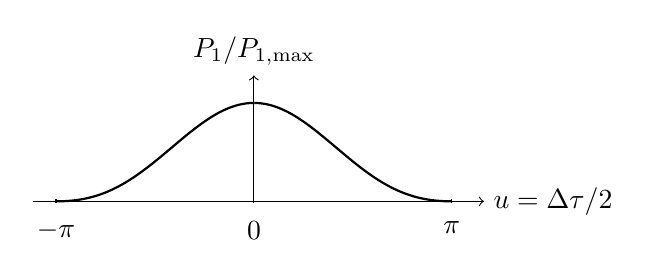
\begin{tikzpicture}[x=0.8cm,y=1.25cm]
\draw[->] (-3.5,0)--(3.65,0) node[right] {$u=\Delta\tau/2$};
\draw[->] (0,0)--(0,1.28) node[above] {$P_1/P_{1,\max}$};
\draw[thick] plot[domain=-pi:-0.01,samples=121] (\x,{(sin(deg(\x))/\x)^2});
\draw[thick] plot[domain=-0.01:0.01,samples=5] (\x,{(1-\x^2/6+\x^4/120)^2});
\draw[thick] plot[domain=0.01:pi,samples=121] (\x,{(sin(deg(\x))/\x)^2});
\foreach \x/\lab in {-pi/{-\pi},0/{0},pi/{\pi}} {\draw (\x,0.02)--(\x,-0.02) node[below=3pt] {$\lab$};}
\end{tikzpicture}
\end{center}

\section*{[2.2] 単一パルスの励起スペクトル}
周波数の離調に対して中央ローブは sinc$^2$ 形であり、両側の最近接零点は共鳴から等距離にある。パルス時間 $\tau$ を長くすると、零点間隔 $4\pi/\tau$ が狭くなる。

\section*{[3.1] 二つのパルスとRamsey干渉}
第一パルス後の回転枠振幅は
\[
a(\tau)=\frac{\omega_1}{2\Delta}(e^{-i\Delta\tau}-1).
\]
自由発展中は $a,b$ が一定である。第二パルス中も同じ実験室位相の回転場が続くので、$\dot a=-i\omega_1e^{-i\Delta t}/2$ を $T$ から $T+\tau$ まで積分すると
\begin{align*}
a(T+\tau)&=a(\tau)+\frac{\omega_1}{2\Delta}(e^{-i\Delta(T+\tau)}-e^{-i\Delta T})\\
&=\frac{\omega_1}{2\Delta}(1+e^{-i\Delta T})(e^{-i\Delta\tau}-1).
\end{align*}
従って
\[
\boxed{P_2(\omega)=\frac{4\omega_1^2}{\Delta^2}\cos^2\!\left(\frac{\Delta T}{2}\right)
\sin^2\!\left(\frac{\Delta\tau}{2}\right)}.
\]
共鳴極限は $P_2(\omega_0)=\omega_1^2\tau^2$ で、弱遷移条件はこの値が十分小さいことを含む。$T\gg\tau$ では sinc$^2$ 包絡内に細い干渉縞が並び、最近接零点は Ramsey 因子から
\[
\boxed{\Omega_1=\omega_0-\frac{\pi}{T},\qquad
\Omega_2=\omega_0+\frac{\pi}{T}},\qquad
\boxed{\Delta\Omega=\frac{2\pi}{T}}.
\]
この線幅で定義する測定精度は、間隔 $T$ を長くすると改善する。規格化スペクトルの模式図は $\tau/T=0.1$ の例で、包絡の最近傍零点より内側にある最初の Ramsey 零点を示す。
\begin{center}
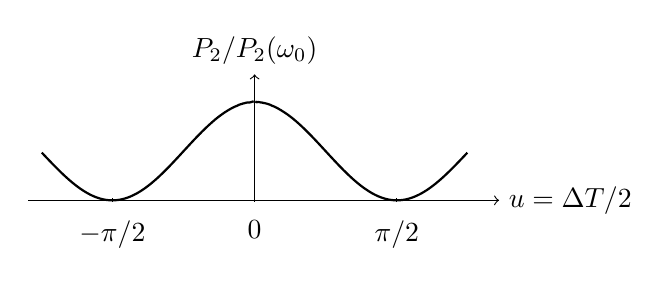
\begin{tikzpicture}[x=1.15cm,y=1.25cm]
\draw[->] (-2.5,0)--(2.7,0) node[right] {$u=\Delta T/2$};
\draw[->] (0,0)--(0,1.28) node[above] {$P_2/P_2(\omega_0)$};
\pgfmathsetmacro{\ratio}{0.1}
\draw[thick] plot[domain=-2.35:-0.01,samples=161] (\x,{cos(deg(\x))^2*(sin(deg(\ratio*\x))/(\ratio*\x))^2});
\draw[thick] plot[domain=-0.01:0.01,samples=5] (\x,{cos(deg(\x))^2*(1-(\ratio*\x)^2/6+(\ratio*\x)^4/120)^2});
\draw[thick] plot[domain=0.01:2.35,samples=161] (\x,{cos(deg(\x))^2*(sin(deg(\ratio*\x))/(\ratio*\x))^2});
\foreach \x/\lab in {{-pi/2}/{-\pi/2},0/0,{pi/2}/{\pi/2}} {\draw (\x,0.02)--(\x,-0.02) node[below=3pt] {$\lab$};}
\end{tikzpicture}
\end{center}

\section*{[4.1] 二重スリットとの対応}
二重スリットの干渉因子の隣接暗線間隔 $\lambda L/l$ に、Ramsey 零点間隔 $2\pi/T$ が対応する。また単スリット包絡の最初の暗線間隔 $2\lambda L/D$ に、パルス包絡の最初の零点間隔 $4\pi/\tau$ が対応する。両者を比較して
\[
\frac{2\pi}{T}\leftrightarrow\frac{\lambda L}{l},\qquad
\frac{4\pi}{\tau}\leftrightarrow\frac{2\lambda L}{D};
\qquad \boxed{T\leftrightarrow l,\quad \tau\leftrightarrow D}.
\]
$T$ は二つのパルス間隔に由来する細かい干渉縞、$\tau$ は有限パルス長に由来する広い回折包絡を決める。

\section*{[4.2] 中間測定による干渉の消失}
中間時刻 $\tau<t<T$ の $z$ 測定で $|+\rangle$ を得る確率は $P_1$、$|-\rangle$ は $1-P_1$ である。測定により二つのパルス間の相対位相は失われる。$|+\rangle$から始める第二パルスでは$a\simeq1$として振幅方程式を使うと、$b(T+\tau)-b(T)=-(i\omega_1/2)\int_T^{T+\tau}e^{i\Delta t}\,dt$である。その絶対値二乗は$P_1$なので、第二パルスはどちらの基底状態からも反対状態への遷移確率が $P_1$ となる。最後に $|+\rangle$ を得る全確率は
\[
P_{\rm meas}=(1-P_1)P_1+P_1(1-P_1)=2P_1(1-P_1)
\simeq2P_1\qquad(P_1\ll1).
\]
従って二重パルスの細かい Ramsey 干渉縞は消え、$P_1(\omega)$ と同じ単一パルスの広い sinc$^2$ 形が残る（高さは弱遷移近似で約2倍）。図は弱遷移近似の $2P_1$ をピークで規格化して描く。
\begin{center}
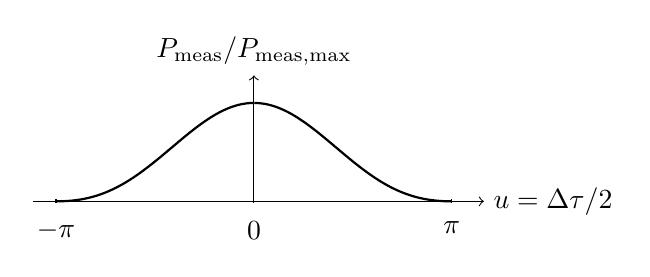
\begin{tikzpicture}[x=0.8cm,y=1.25cm]
\draw[->] (-3.5,0)--(3.65,0) node[right] {$u=\Delta\tau/2$};
\draw[->] (0,0)--(0,1.28) node[above] {$P_{\rm meas}/P_{{\rm meas},\max}$};
\draw[thick] plot[domain=-pi:-0.01,samples=121] (\x,{(sin(deg(\x))/\x)^2});
\draw[thick] plot[domain=-0.01:0.01,samples=5] (\x,{(1-\x^2/6+\x^4/120)^2});
\draw[thick] plot[domain=0.01:pi,samples=121] (\x,{(sin(deg(\x))/\x)^2});
\foreach \x/\lab in {-pi/{-\pi},0/{0},pi/{\pi}} {\draw (\x,0.02)--(\x,-0.02) node[below=3pt] {$\lab$};}
\end{tikzpicture}
\end{center}
\end{document}
